\chapter{Plant Vegetative Development: Meristems and Growth}\label{ch:b2:plant-meristems}

An oak that was a seedling when the cathedral was built is still
adding a ring of \omterm{def:b2:plant-meristems:wood}{wood} every year, still opening new leaves every
spring, still pushing new root tips through the soil. No animal does
this; a horse stops growing at four. The difference is that a plant
keeps, at the tip of every shoot and every root and in a thin
cylinder inside every trunk, small populations of embryonic cells
--- the \emph{\omterm{def:b2:plant-meristems:meristem}{meristems}} --- that never stop dividing, and that build
the plant's body outward and upward for as long as it lives. This
chapter looks at how the two apical \omterm{def:b2:plant-meristems:meristem}{meristems} are organised and
controlled, how a plant cell grows, how hormones decide the shape of
a shoot, and how a trunk thickens.

\section{Meristems}

\begin{definition}[Meristems and the two kinds of growth]\label{def:b2:plant-meristems:meristem}
\index{meristem}\index{shoot apical meristem}\index{root apical meristem}\index{cambium}
A \emph{meristem} is a population of small, undifferentiated,
dividing cells that persists throughout the plant's life and from
which all its tissues derive. The \emph{shoot apical meristem} (SAM)
at the tip of each shoot makes leaves, stem and, in season, \omterm{def:b2:angiosperm-reproduction:flower}{flowers};
the \emph{root apical meristem} (RAM) behind each root tip makes the
root; together they drive \emph{primary growth}, the lengthening of
the plant. The \emph{lateral meristems} --- the \emph{\omterm{def:b2:plant-meristems:wood}{vascular
cambium}} and the \emph{cork cambium}, thin cylinders inside stems
and roots --- drive \emph{secondary growth}, the thickening that
makes \omterm{def:b2:plant-meristems:wood}{wood} and \omterm{def:b2:plant-meristems:wood}{bark}. Plant growth is therefore \emph{indeterminate}:
the meristems can go on indefinitely, and the plant is a modular
organism, repeating the unit leaf--node--internode--bud as long as
conditions allow. Every axillary bud is a dormant SAM, so a plant
carries thousands of reserve growing points.
\end{definition}

\begin{proposition}[The shoot apex]\label{prop:b2:plant-meristems:sam}
\index{phyllotaxis}\index{leaf primordium}\index{plastochron}
The SAM is a dome a tenth of a millimetre across, of a few hundred
cells. Its outer one or two layers (the \emph{tunica}) divide only
in the plane of the surface and give the epidermis; the mass below
(the \emph{corpus}) divides in all planes. At the summit a
\emph{central zone} of slowly dividing \omterm{def:b2:cell-differentiation:differentiation}{stem cells} feeds a
\emph{peripheral zone} of faster-dividing cells, where \emph{leaf
primordia} arise as bulges at regular intervals of time (the
\emph{plastochron}, hours to days) and at regular angles around the
dome (the \emph{phyllotaxis}: opposite, whorled, or spiral at the
golden angle of \qty{137.5}{\degree}, which places each new leaf in
the largest gap left by the others). Below, a \emph{rib zone} makes
the pith and lengthens the stem. A primordium forms where the
hormone auxin accumulates in the surface layer, and as it grows it
drains auxin from its surroundings, which is why the next
primordium arises as far from it as possible: the pattern is
self-organising.
\end{proposition}

\begin{omfigure}
\begin{tikzpicture}[every node/.style={font=\scriptsize}]
  % dome
  \draw[thick, fill=omExo!12] (-2.2,0) .. controls (-2.2,1.6) and (-0.8,2.6) .. (0,2.6) .. controls (0.8,2.6) and (2.2,1.6) .. (2.2,0) -- (2.2,-1.4) -- (-2.2,-1.4) -- cycle;
  % tunica layers
  \draw[thick, omDef] (-2.2,0) .. controls (-2.2,1.5) and (-0.8,2.45) .. (0,2.45) .. controls (0.8,2.45) and (2.2,1.5) .. (2.2,0);
  \draw[thick, omDef] (-2.05,0) .. controls (-2.05,1.35) and (-0.75,2.3) .. (0,2.3) .. controls (0.75,2.3) and (2.05,1.35) .. (2.05,0);
  % zones
  \draw[thick, dashed, omThm, fill=omThm!15] (0,1.75) ellipse (0.6 and 0.55);
  \draw[thick, dashed, omProp] (0,0.9) ellipse (1.6 and 1.35);
  \draw[thick, dashed, omExo!70!black] (-0.9,-0.9) rectangle (0.9,-0.1);
  % primordia
  \draw[thick, fill=omExo!40] (-2.2,0.4) .. controls (-2.5,1.4) and (-1.6,1.9) .. (-1.55,1.3) .. controls (-1.5,0.9) and (-1.9,0.6) .. (-2.2,0.4);
  \draw[thick, fill=omExo!40] (2.2,0.2) .. controls (2.7,1.0) and (2.1,1.5) .. (1.75,1.1) .. controls (1.6,0.8) and (1.9,0.5) .. (2.2,0.2);
  % labels
  \draw (0.4,2.1) -- (3.2,2.6) node[right, align=left] {central zone:\\slowly dividing stem cells};
  \draw (1.3,0.5) -- (3.2,1.4) node[right, align=left] {peripheral zone:\\fast division, leaf primordia};
  \draw (0.6,-0.5) -- (3.2,0.0) node[right, align=left] {rib zone: pith,\\stem elongation};
  \draw (-1.7,1.5) -- (-3.0,2.4) node[left, align=right] {leaf\\primordium};
  \draw (-1.2,2.05) -- (-3.0,1.2) node[left, align=right] {tunica: surface\\divisions only};
  \draw (2.2,0.7) -- (3.2,-1.0) node[right, align=left] {next primordium,\\\qty{137.5}{\degree} round};
\end{tikzpicture}

{\small The \omterm{def:b2:plant-meristems:meristem}{shoot apical meristem} in section: a tunica of one or two
surface layers over a corpus, a central zone of \omterm{def:b2:cell-differentiation:differentiation}{stem cells} at the
summit, a peripheral zone where leaf primordia bulge out, and a rib
zone below.}
\end{omfigure}

\begin{omfigure}
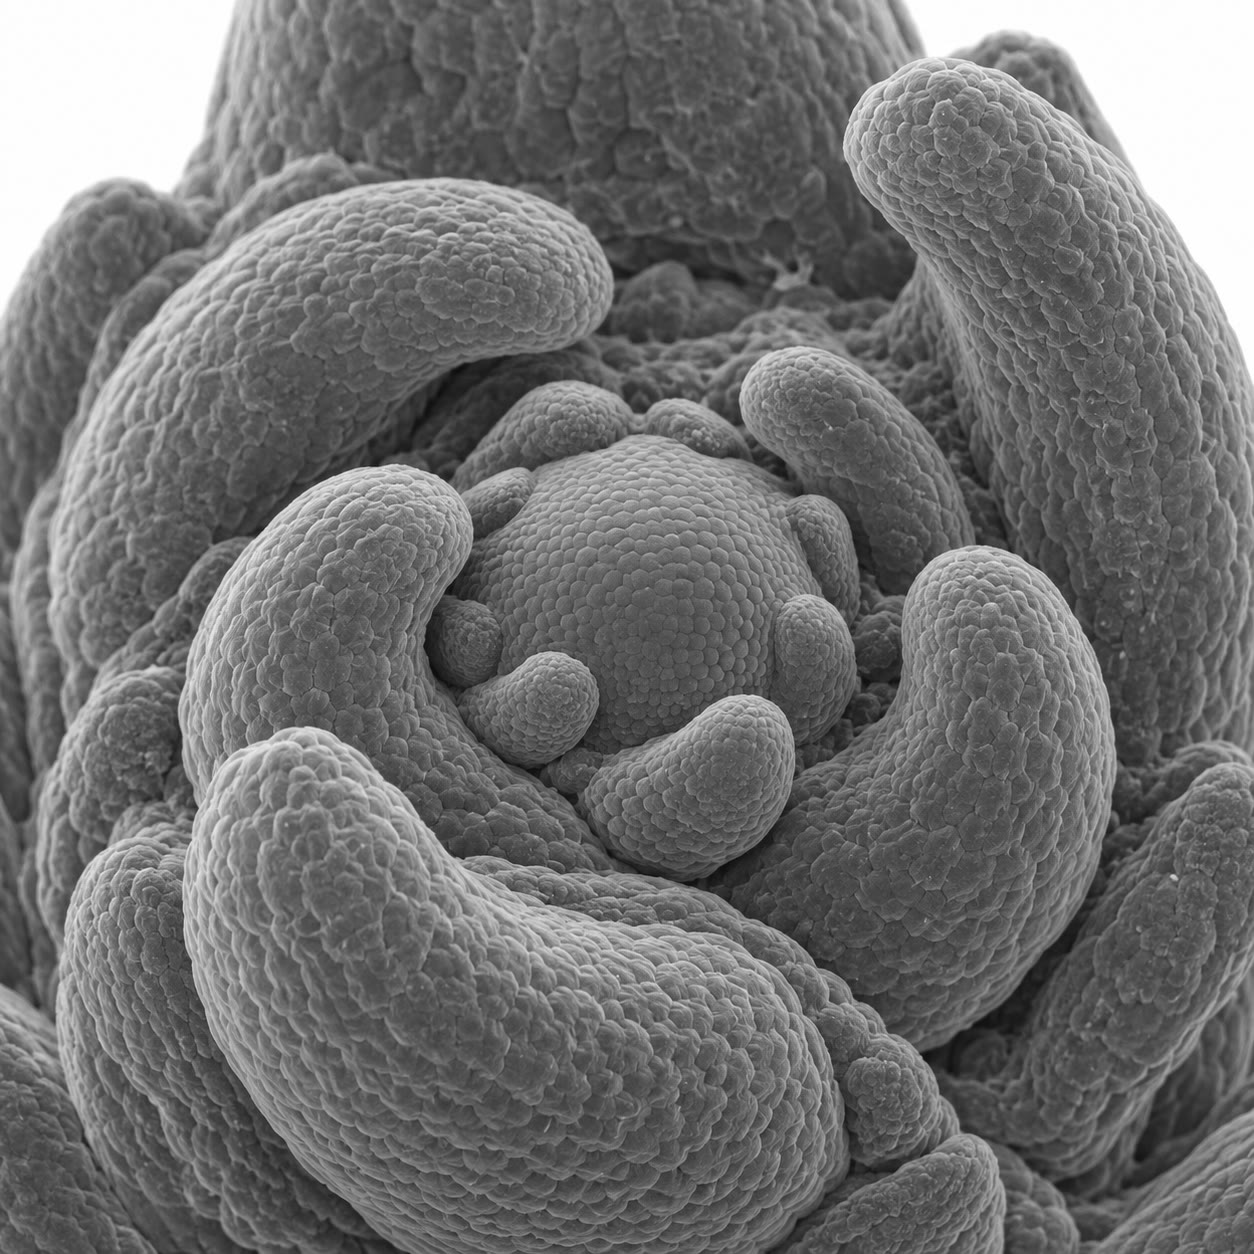
\includegraphics[width=0.44\linewidth]{images/book4/ai/b4-13-shoot-apex-sem.jpg}

{\small A shoot apex under the scanning electron microscope: the
smooth dome of the \omterm{def:b2:plant-meristems:meristem}{meristem} and the spiral of leaf primordia around
it, each new one placed in the widest gap.}
\end{omfigure}

\begin{proposition}[Keeping the stem cells: a feedback loop]\label{prop:b2:plant-meristems:wus}
\index{WUSCHEL}\index{CLAVATA}\index{negative feedback!meristem}
The size of the stem-cell pool is held constant by a loop between
two genes. Cells just beneath the central zone express the
\omterm{prop:b2:cell-differentiation:transcriptional}{transcription factor} \emph{WUSCHEL} (WUS), whose product moves up
into the overlying cells and keeps them as \omterm{def:b2:cell-differentiation:differentiation}{stem cells}; the \omterm{def:b2:cell-differentiation:differentiation}{stem
cells} in turn secrete a small peptide, \emph{CLAVATA3} (CLV3), that
diffuses down, binds a receptor kinase (CLV1) in the WUS-expressing
cells and represses WUS. More \omterm{def:b2:cell-differentiation:differentiation}{stem cells} means more CLV3, less WUS,
fewer \omterm{def:b2:cell-differentiation:differentiation}{stem cells}; fewer \omterm{def:b2:cell-differentiation:differentiation}{stem cells} means less CLV3, more WUS, more
\omterm{def:b2:cell-differentiation:differentiation}{stem cells}. The pool is thus a regulated quantity, like the
gonadotropins of \cref{ch:b2:reproductive-hormones}, and the same
logic --- a signal from the regulated population repressing the
factor that makes it --- holds the root \omterm{def:b2:plant-meristems:meristem}{meristem} too.
\end{proposition}
\begin{proof}[Evidence]
Arabidopsis \emph{clavata} mutants (Clark, Meyerowitz, 1990s) have
\omterm{def:b2:plant-meristems:meristem}{meristems} that swell to many times the normal size, with extra
leaves, extra floral organs and fasciated (flattened, ribbon-like)
stems: the brake is gone. \emph{wuschel} mutants make a \omterm{def:b2:plant-meristems:meristem}{meristem}
that stops after a few leaves and then forms new ones, each of which
stops in turn: the accelerator is gone. In the double mutant the
\emph{wuschel} \omterm{def:b2:meiosis-heredity:vocabulary}{phenotype} prevails, placing WUS downstream of CLV;
and CLV3 peptide applied to a wild-type apex represses WUS within
hours.
\end{proof}

\begin{proposition}[The root apex]\label{prop:b2:plant-meristems:ram}
\index{root cap}\index{quiescent centre}\index{elongation zone}\index{root hair}
A root grows from a \omterm{def:b2:plant-meristems:meristem}{meristem} sheltered behind a \emph{\omterm{prop:b2:plant-meristems:ram}{root cap}},
whose cells are sloughed off as the tip pushes through the soil and
which secretes a lubricating mucilage and senses gravity (starch
grains that settle in its cells). At the centre of the \omterm{def:b2:plant-meristems:meristem}{meristem} a
\emph{\omterm{prop:b2:plant-meristems:ram}{quiescent centre}} of a few hundred cells divides only rarely;
it keeps the surrounding initials --- of the cap, the epidermis, the
cortex and the vascular cylinder --- as \omterm{def:b2:cell-differentiation:differentiation}{stem cells}, much as WUS
keeps the shoot's. Behind the \omterm{def:b2:plant-meristems:meristem}{meristem} comes the \emph{\omterm{prop:b2:plant-meristems:ram}{elongation
zone}}, a few millimetres in which cells lengthen ten- to
twentyfold, driving the tip forward; then the \emph{\omterm{def:b2:cell-differentiation:differentiation}{differentiation}
zone}, where the epidermis grows \emph{\omterm{prop:b2:plant-meristems:ram}{root hairs}} and xylem and
phloem mature. Lateral roots arise not at the tip but from the
pericycle, deep inside the mature root, opposite the xylem poles,
and push out through the cortex. Auxin, made in the shoot and
carried down, accumulates at the tip and organises the whole
arrangement; the \omterm{prop:b2:plant-meristems:ram}{quiescent centre} sits at its maximum.
\end{proposition}

\begin{omfigure}
\begin{tikzpicture}[every node/.style={font=\scriptsize}]
  % root outline
  \draw[thick, fill=omExo!10] (-1.0,4.5) -- (-1.0,0.6) .. controls (-1.0,-0.4) and (1.0,-0.4) .. (1.0,0.6) -- (1.0,4.5);
  % root cap
  \draw[thick, fill=omExo!45] (-0.9,0.8) .. controls (-1.1,-0.1) and (1.1,-0.1) .. (0.9,0.8) .. controls (0.5,0.4) and (-0.5,0.4) .. (-0.9,0.8);
  % meristem
  \fill[omThm!25] (-0.85,0.8) rectangle (0.85,1.7);
  \fill[omThm!70] (0,0.95) ellipse (0.25 and 0.12);
  % elongation zone
  \fill[omProp!20] (-0.85,1.7) rectangle (0.85,3.0);
  % differentiation zone with root hairs and vascular strand
  \fill[omDef!15] (-0.85,3.0) rectangle (0.85,4.5);
  \fill[omDef!50] (-0.15,3.0) rectangle (0.15,4.5);
  \foreach \y in {3.2,3.5,3.8,4.1,4.4} { \draw[omDef!80!black] (1.0,\y) -- (1.7,\y+0.1); \draw[omDef!80!black] (-1.0,\y) -- (-1.7,\y+0.1); }
  % lateral root primordium
  \draw[thick, fill=omThm!30] (0.15,4.0) .. controls (0.5,3.9) and (0.8,4.1) .. (0.9,4.3) .. controls (0.7,4.35) and (0.4,4.3) .. (0.15,4.3);
  % labels
  \draw (0.5,0.4) -- (2.2,0.2) node[right] {root cap};
  \draw (0.25,0.95) -- (2.2,0.9) node[right] {quiescent centre};
  \draw (0.85,1.4) -- (2.2,1.5) node[right] {meristem (division)};
  \draw (0.85,2.4) -- (2.2,2.3) node[right, align=left] {elongation zone:\\cells lengthen $10\times$};
  \draw (1.5,3.6) -- (2.2,3.4) node[right] {root hairs};
  \draw (0.0,4.2) -- (2.2,4.2) node[right] {vascular cylinder};
  \draw (0.7,4.3) -- (2.2,4.9) node[right, align=left] {lateral root primordium\\(from the pericycle)};
  \draw[->, thick] (-2.4,4.5) -- (-2.4,0.6); \node[left, rotate=90, anchor=south] at (-2.5,2.5) {auxin flows to the tip};
\end{tikzpicture}

{\small The root tip: cap, \omterm{def:b2:plant-meristems:meristem}{meristem} with its \omterm{prop:b2:plant-meristems:ram}{quiescent centre},
\omterm{prop:b2:plant-meristems:ram}{elongation zone}, and the \omterm{def:b2:cell-differentiation:differentiation}{differentiation} zone with \omterm{prop:b2:plant-meristems:ram}{root hairs} and
mature vessels. Lateral roots start deep inside, from the pericycle.}
\end{omfigure}

\begin{omfigure}
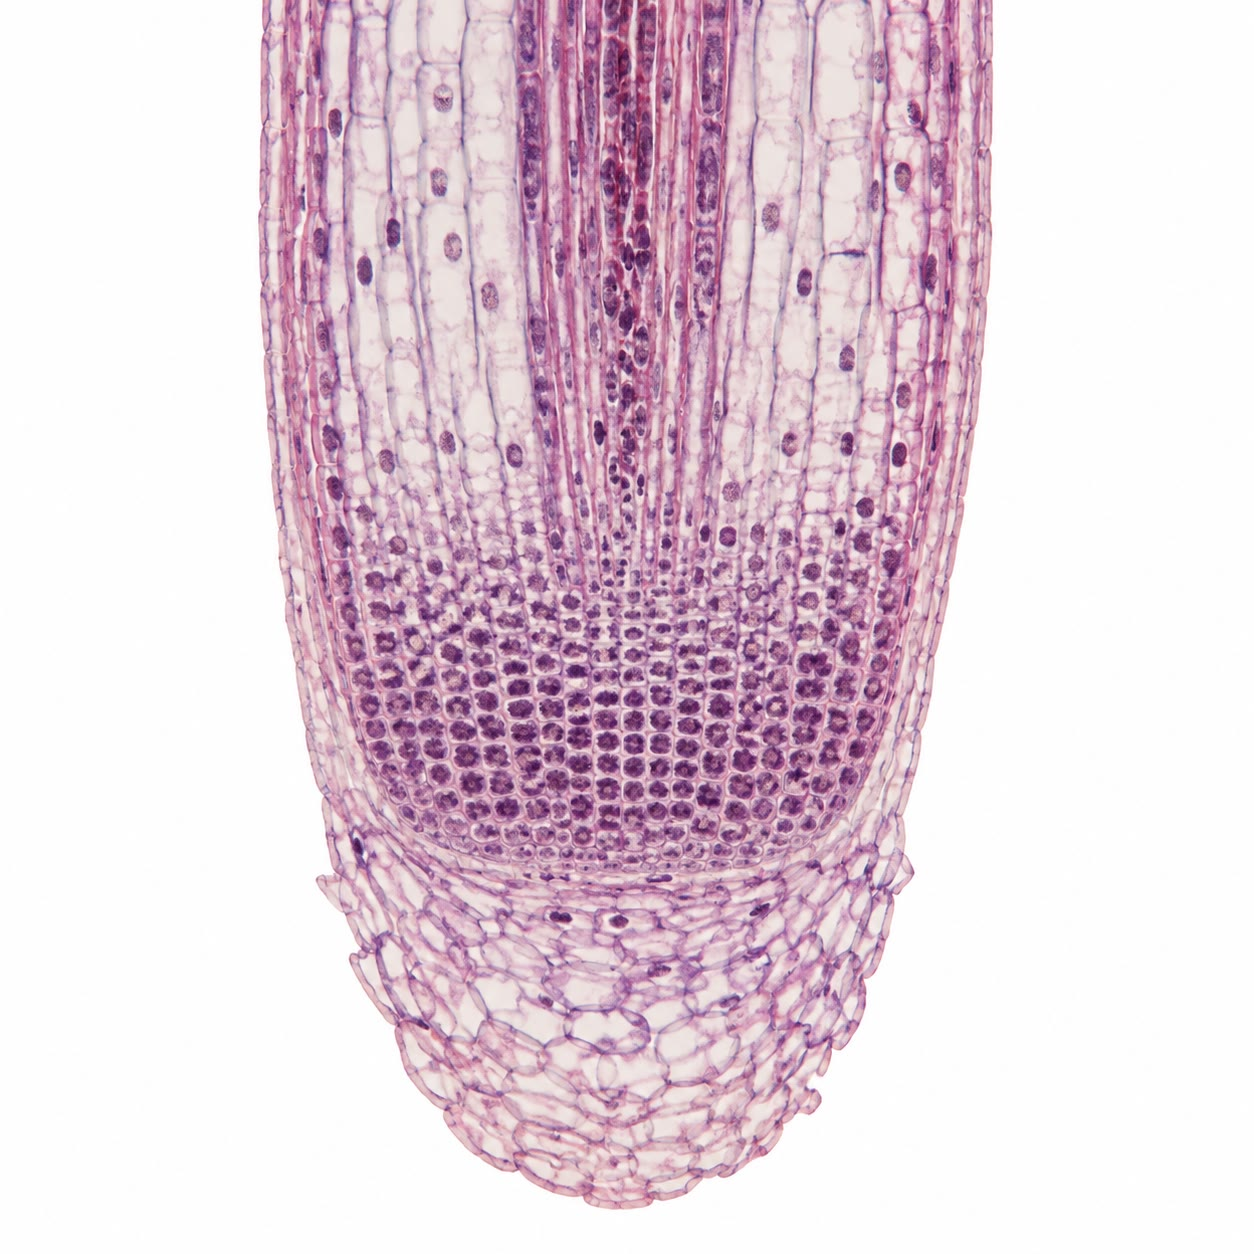
\includegraphics[width=0.42\linewidth]{images/book4/ai/b4-13-root-tip.jpg}

{\small A root tip in longitudinal section: the loose cells of the
cap, the dense \omterm{def:b2:plant-meristems:meristem}{meristem} with its dark nuclei, and the lengthening
cells above.}
\end{omfigure}

\section{How a plant cell grows}

\begin{theorem}[Lockhart's equation]\label{thm:b2:plant-meristems:lockhart}
\index{turgor}\index{cell wall!extensibility}\index{Lockhart equation}
A plant cell grows by stretching its wall under the pressure of its
own contents. The wall yields irreversibly only above a threshold
turgor $Y$, and then at a rate proportional to the excess: the
relative growth rate of a cell of length $L$ is
\[
\frac{1}{L}\frac{\mathrm{d}L}{\mathrm{d}t} = \phi\,(P - Y) \quad (P > Y),
\]
where $P$ is the turgor pressure and $\phi$ the wall's
\emph{extensibility}. Growth is therefore controlled from two sides:
by water, which sets $P$ (a wilting cell stops growing), and by the
wall, which sets $\phi$ and $Y$ --- and it is the wall that hormones
act on. Auxin makes cells pump protons into the wall; the acid
activates \emph{expansins}, proteins that loosen the bonds between
cellulose fibrils and the matrix, raising $\phi$ and lowering $Y$
within minutes (\emph{acid growth}). With $\phi =
\qty{0.1}{h^{-1}.MPa^{-1}}$, $Y = \qty{0.3}{MPa}$ and $P =
\qty{0.6}{MPa}$, a cell lengthens by \qty{3}{\%} an hour and doubles
in a day; in a root's \omterm{prop:b2:plant-meristems:ram}{elongation zone}, where the rates are several
times higher, a cell lengthens tenfold in a few hours.
\end{theorem}
\begin{proof}
The wall is a viscoplastic material: below the yield stress it
deforms elastically and recovers, above it flows at a rate
proportional to the excess stress. The stress in the wall is
proportional to the turgor pressure (for a cylinder of radius $r$
and wall thickness $w$, the hoop stress is $Pr/w$), so the plastic
strain rate is proportional to $P - Y$ with a constant $\phi$ that
absorbs the geometry and the wall's material properties. The strain
rate is by definition $(1/L)\,\mathrm{d}L/\mathrm{d}t$. Numerically,
$0.1\times(0.6 - 0.3) = \qty{0.03}{h^{-1}}$, and $L$ doubles when
$0.03\,t = \ln 2$, $t = \qty{23}{h}$.
\end{proof}

\begin{omfigure}
\begin{tikzpicture}
\begin{axis}[
  width=0.7\linewidth, height=5.4cm,
  axis x line=bottom, axis y line=left,
  xmin=0, xmax=1.0, ymin=0, ymax=0.09,
  xlabel={turgor pressure $P$ (\unit{MPa})}, ylabel={relative growth rate (\unit{h^{-1}})},
  xlabel style={font=\small, at={(axis description cs:0.5,-0.13)}, anchor=north},
  ylabel style={font=\small},
  tick label style={font=\small}, xtick={0,0.3,0.6,0.9}, ytick={0,0.03,0.06,0.09},
  yticklabels={0,0.03,0.06,0.09}, scaled y ticks=false,
  legend style={font=\scriptsize, at={(0.03,0.97)}, anchor=north west, draw=none},
  clip=false,
]
\addplot[very thick, omDef, domain=0:0.3, samples=2, forget plot] {0};
\addplot[very thick, omDef, domain=0.3:1.0, samples=2] {0.1*(x-0.3)};
\addlegendentry{$\phi = 0.1$, $Y = 0.3$}
\addplot[very thick, omThm, domain=0:0.2, samples=2, forget plot] {0};
\addplot[very thick, omThm, domain=0.2:0.65, samples=2] {0.2*(x-0.2)};
\addlegendentry{with auxin: $\phi = 0.2$, $Y = 0.2$}
\draw[dashed, gray] (axis cs:0.6,0) -- (axis cs:0.6,0.03); \node[font=\scriptsize, anchor=west] at (axis cs:0.61,0.015) {typical $P$};
\end{axis}
\end{tikzpicture}

{\small Lockhart's law: no growth below the yield turgor, then a
rate proportional to the excess. Auxin, by loosening the wall,
lowers the threshold and steepens the line, and at the same turgor
the cell grows several times faster.}
\end{omfigure}

\begin{example}[Where the water comes from]\label{ex:b2:plant-meristems:water}
As the wall yields, the turgor would fall and growth stop, were
water not entering to keep pace: the growing cell is a leak that
refills itself. The water comes from the xylem, down a small
gradient of water potential, and its rate of entry is set by the
membrane's hydraulic conductance; growth is fastest at night, when
transpiration is low and turgor high, and a maize leaf can extend
\qty{10}{cm} between dusk and dawn. Under drought the cells make
solutes (\emph{osmotic adjustment}) to keep $P$ above $Y$, and when
that fails the leaf stops growing days before it wilts.
\end{example}

\section{Hormones and the shape of the shoot}

\begin{proposition}[Auxin and apical dominance]\label{prop:b2:plant-meristems:apical}
\index{auxin}\index{apical dominance}\index{polar auxin transport}\index{cytokinin}
\emph{Auxin} (indole-3-acetic acid) is made in the shoot apex and
young leaves and carried down the stem, cell to cell, at about
\qty{1}{cm/h}, by carrier proteins (PIN) set into the lower end of
each cell --- a \emph{polar transport} that gives the plant a
top-to-bottom axis. The stream of auxin descending from the apex
keeps the axillary buds below it dormant (\emph{\omterm{prop:b2:plant-meristems:apical}{apical dominance}}),
in part by preventing them from exporting their own auxin into the
stem, in part by inducing strigolactones and repressing cytokinin.
Cut off the apex and the buds nearest the cut grow out within days,
making a bushy plant --- which is what pruning and pinching exploit.
\emph{Cytokinins}, made in the root tips and carried up in the xylem,
promote bud outgrowth and cell division; \emph{gibberellins}
lengthen internodes (dwarf peas and the semi-dwarf wheat of the
Green Revolution are defective in making or sensing them); abscisic
acid and ethylene brake growth under stress. The shoot's form ---
tall or bushy, upright or spreading --- is a negotiation among
these signals, and the root-to-shoot balance is set by the auxin
going down against the cytokinin coming up.
\end{proposition}
\begin{proof}[Evidence]
Thimann and Skoog (1934) cut the apex from bean plants: the lateral
buds grew. A block of agar containing auxin, placed on the cut
stump, kept them dormant as the apex had; plain agar did not. Went
(1928) had already measured auxin by the bend it produced in
decapitated oat coleoptiles when placed on one side of the stump ---
the first bioassay of a plant hormone, and the origin of the name,
from the Greek for ``to grow''. The polarity of transport was shown
by placing auxin agar on one end of a stem segment and finding it
in a receiver block at the other end only when the segment was
oriented apex-up, however the segment was turned in the gravity
field.
\end{proof}

\begin{omfigure}
\begin{tikzpicture}[every node/.style={font=\scriptsize}, >=stealth]
  \foreach \x/\lab/\apex/\aux in {0/{intact: apex on,\\buds dormant}/1/0, 4.2/{decapitated:\\buds grow out}/0/0, 8.4/{decapitated + auxin\\on the stump: dormant}/0/1} {
    \begin{scope}[xshift=\x cm]
      \draw[very thick, omExo!70!black] (0,0) -- (0,3.4);
      \foreach \y in {0.8,1.6,2.4} { \draw[thick, omExo!70!black] (0,\y) -- (-0.8,\y+0.4); \draw[thick, omExo!70!black] (0,\y+0.4) -- (0.8,\y+0.8); }
      \ifnum\apex=1 \draw[thick, fill=omThm!40] (0,3.5) ellipse (0.25 and 0.3); \draw[->, thick, omThm] (0.35,3.2) -- (0.35,1.0); \node[omThm, right] at (0.4,2.1) {auxin}; \fi
      \ifnum\apex=0 \draw[thick] (-0.3,3.4) -- (0.3,3.4); \fi
      \ifnum\aux=1 \draw[thick, fill=omThm!40] (-0.25,3.4) rectangle (0.25,3.75); \node[omThm, right] at (0.3,3.6) {auxin agar}; \draw[->, thick, omThm] (0.35,3.2) -- (0.35,1.0); \fi
      \ifnum\apex=1 \foreach \y in {0.8,1.6,2.4} \fill[gray!60] (-0.12,\y+0.1) circle (0.08); \fi
      \ifnum\aux=1 \foreach \y in {0.8,1.6,2.4} \fill[gray!60] (-0.12,\y+0.1) circle (0.08); \fi
      \ifnum\apex=0 \ifnum\aux=0 \foreach \y in {0.8,1.6,2.4} { \draw[thick, omExo!70!black] (-0.1,\y+0.1) -- (-0.7,\y+0.9); \draw[thick, omExo!70!black] (-0.7,\y+0.9) -- (-1.0,\y+1.1); \draw[thick, omExo!70!black] (-0.7,\y+0.9) -- (-0.75,\y+1.25); } \fi\fi
      \node[below, align=center] at (0,-0.3) {\lab};
    \end{scope}
  }
\end{tikzpicture}

{\small \omterm{prop:b2:plant-meristems:apical}{Apical dominance}, the Thimann--Skoog experiment. The apex
keeps the axillary buds dormant; removing it releases them; auxin on
the cut stump replaces the apex.}
\end{omfigure}

\begin{example}[Fast signal, slow molecule]\label{ex:b2:plant-meristems:transport}
Polar transport moves auxin \qty{1}{cm} in an hour; diffusion alone
would take, for the same centimetre, $t = x^2/2D = 10^{-4}/(2\times
10^{-9}) = \qty{5e4}{s}$ --- fourteen hours --- and for the ten
centimetres to a lower bud, sixty days. The pump-and-relay of the
PIN carriers is what makes a hormonal signal usable over the length
of a plant; the same carriers, moved to the shaded side of a stem,
bend it toward the light (\cref{ch:b2:plant-plasticity}).
\end{example}

\section{Secondary growth: wood and bark}

\begin{definition}[The vascular cambium and wood]\label{def:b2:plant-meristems:wood}
\index{vascular cambium}\index{wood}\index{annual ring}\index{bark}\index{periderm}
In a woody stem the strands of primary xylem and phloem are joined,
in the first year, into a continuous cylinder of dividing cells,
the \emph{vascular \omterm{def:b2:plant-meristems:meristem}{cambium}}. Its cells divide tangentially, adding
\emph{secondary xylem} --- \emph{wood} --- to the inside and
\emph{secondary phloem} to the outside, so that the \omterm{def:b2:plant-meristems:meristem}{cambium} moves
outward as the trunk thickens, and adding occasional radial
divisions to widen the ring. In seasonal climates the wood laid down
in spring has wide, thin-walled vessels (\emph{earlywood}) and that
of summer narrow, thick-walled ones (\emph{latewood}), so that each
year leaves a visible \emph{annual ring}; the rings record the
tree's age and, in their widths, the climate of each year
(dendrochronology). Only the outer rings, the \emph{sapwood},
conduct; the inner ones, the \emph{heartwood}, are dead, plugged
and darkened with resins and tannins, and serve as the tree's
skeleton. Outside the phloem a second lateral \omterm{def:b2:plant-meristems:meristem}{meristem}, the
\emph{cork \omterm{def:b2:plant-meristems:meristem}{cambium}}, makes the \emph{periderm} --- layers of cork
cells, dead and waterproofed with suberin --- which with the old
phloem is the \emph{bark}. A trunk is thus a thin living shell of
\omterm{def:b2:plant-meristems:meristem}{cambium}, sapwood and phloem around a dead core, under a dead skin.
\end{definition}

\begin{omfigure}
\begin{tikzpicture}[every node/.style={font=\scriptsize}]
  \fill[omExo!60] (0,0) circle (3.0);
  \fill[omDef!20] (0,0) circle (2.75);
  \fill[omDef!35] (0,0) circle (2.2);
  \foreach \r in {0.4,0.7,1.0,1.3,1.6,1.9,2.2} \draw[omDef!80!black, thin] (0,0) circle (\r);
  \fill[omExo!80!black] (0,0) circle (1.3);
  \foreach \r in {0.4,0.7,1.0} \draw[omExo!40, thin] (0,0) circle (\r);
  \draw[very thick, omThm] (0,0) circle (2.5);
  \draw (2.9,0.6) -- (3.9,1.6) node[right, align=left] {bark: cork (periderm)\\and old phloem};
  \draw (2.62,0.0) -- (3.9,0.6) node[right] {secondary phloem, living};
  \draw (2.5,-0.4) -- (3.9,-0.4) node[right] {vascular cambium (red)};
  \draw (1.9,-1.1) -- (3.9,-1.4) node[right, align=left] {sapwood: recent rings,\\conducting};
  \draw (0.5,-0.9) -- (3.9,-2.4) node[right, align=left] {heartwood: old rings,\\dead, plugged};
  \draw (-1.7,1.5) -- (-3.6,2.4) node[left, align=right] {one annual ring:\\pale earlywood,\\dark latewood};
\end{tikzpicture}

{\small A trunk in cross-section. The \omterm{def:b2:plant-meristems:meristem}{cambium} (red) adds \omterm{def:b2:plant-meristems:wood}{wood} inward
and phloem outward each year; the recent rings conduct, the old ones
form the dead heartwood; cork and old phloem make the \omterm{def:b2:plant-meristems:wood}{bark}.}
\end{omfigure}

\begin{theorem}[Why an old tree adds more wood]\label{thm:b2:plant-meristems:rings}
A trunk of radius $r$ and height $h$ whose \omterm{def:b2:plant-meristems:meristem}{cambium} adds a ring of
thickness $\Delta r$ each year gains a volume of \omterm{def:b2:plant-meristems:wood}{wood}
\[
\Delta V \approx 2\pi r\,h\,\Delta r
\]
per year: for a constant ring width, the annual increment grows in
proportion to the radius, and a tree of \qty{50}{cm} radius adds ten
times the \omterm{def:b2:plant-meristems:wood}{wood} of one with \qty{5}{cm}, though its rings are no
wider. A trunk of \qty{25}{cm} radius and \qty{10}{m} height adding
\qty{4}{mm} a year gains \qty{0.063}{m^3}, about \qty{30}{kg} of dry
\omterm{def:b2:plant-meristems:wood}{wood} --- \qty{15}{kg} of carbon, drawn from the air by the crown in
one season.
\end{theorem}
\begin{proof}
The \omterm{def:b2:plant-meristems:wood}{wood} added is a cylindrical shell of circumference $2\pi r$,
thickness $\Delta r$ and height $h$; its volume is $2\pi r h\Delta r$
to first order in $\Delta r$ (exactly $\pi h[(r + \Delta r)^2 - r^2]
= \pi h(2r\Delta r + \Delta r^2)$). With $r = 0.25$, $h = 10$,
$\Delta r = 0.004$: $2\pi\times 0.25\times 10\times 0.004 =
\qty{0.063}{m^3}$; at \qty{500}{kg/m^3} dry, \qty{31}{kg}, half of it
carbon.
\end{proof}

\begin{omfigure}
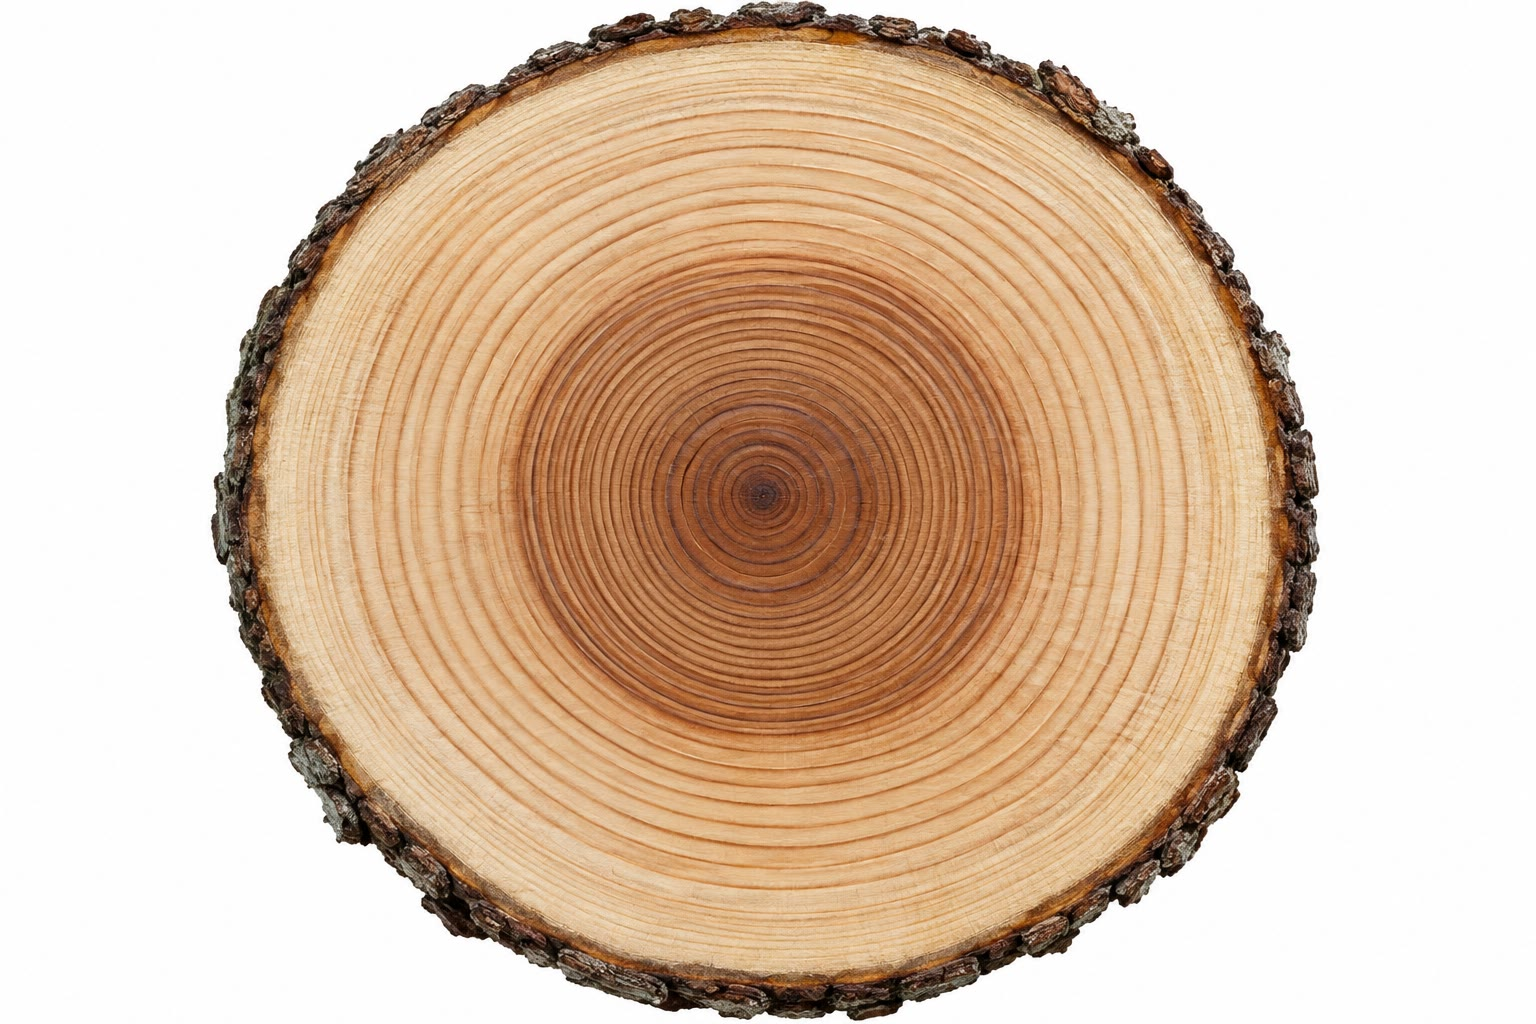
\includegraphics[width=0.5\linewidth]{images/book4/ai/b4-13-wood-rings.jpg}

{\small A pine trunk in cross-section: the \omterm{def:b2:plant-meristems:wood}{annual rings}, each a pale
band of earlywood and a dark band of latewood, the darker heartwood,
and the \omterm{def:b2:plant-meristems:wood}{bark}.}
\end{omfigure}

\section{Exercises}

\begin{exercise}[$\star$]\label{exo:b2:plant-meristems:1}
Define \omterm{def:b2:plant-meristems:meristem}{meristem}, and name the four \omterm{def:b2:plant-meristems:meristem}{meristems} of a woody plant with
what each produces.
\end{exercise}

\begin{exercise}[$\star$]\label{exo:b2:plant-meristems:2}
List the zones of a root tip from the cap upward, with what happens
to a cell in each. Where do lateral roots come from?
\end{exercise}

\begin{exercise}[$\star$]\label{exo:b2:plant-meristems:3}
Describe the Thimann--Skoog experiment, its control, and its
conclusion.
\end{exercise}

\begin{exercise}[$\star$]\label{exo:b2:plant-meristems:4}
A trunk section shows 60 rings, the outer 15 pale and the rest dark.
Give the age of the tree, the age of its sapwood, and say which part
of the trunk is alive.
\end{exercise}

\begin{exercise}[$\star\star$]\label{exo:b2:plant-meristems:5}
With $\phi = \qty{0.1}{h^{-1}.MPa^{-1}}$, $Y = \qty{0.3}{MPa}$, compute
the relative growth rate at $P = 0.4$, $0.6$ and \qty{0.8}{MPa}, and
the doubling time at each. A drought lowers $P$ to \qty{0.25}{MPa}:
what happens?
\end{exercise}

\begin{exercise}[$\star\star$]\label{exo:b2:plant-meristems:6}
Successive leaves arise at \qty{137.5}{\degree} from one another.
Compute the angular positions of leaves 1 to 8 (modulo
\qty{360}{\degree}) and show that no two of the first eight lie
within \qty{20}{\degree} of each other. Why does this matter to the
plant?
\end{exercise}

\begin{exercise}[$\star\star$]\label{exo:b2:plant-meristems:7}
A tree \qty{12}{m} tall adds rings of \qty{3}{mm}. Compute the \omterm{def:b2:plant-meristems:wood}{wood}
added in the year its radius is \qty{5}{cm} and in the year it is
\qty{40}{cm}, and the corresponding carbon (dry density
\qty{500}{kg/m^3}, half carbon).
\end{exercise}

\begin{exercise}[$\star\star$]\label{exo:b2:plant-meristems:8}
Predict the \omterm{def:b2:meiosis-heredity:vocabulary}{phenotypes} of a \emph{clv3} mutant, a \emph{wus} mutant,
and the double mutant, and explain the order of the two genes in the
loop from the double mutant.
\end{exercise}

\begin{exercise}[$\star\star$]\label{exo:b2:plant-meristems:9}
Auxin is transported at \qty{1}{cm/h}; its diffusion coefficient in
tissue is \qty{1e-9}{m^2/s}. How long does the signal take to reach
a bud \qty{20}{cm} below the apex by transport, and by diffusion
($t = x^2/2D$)? What does polar transport buy the plant?
\end{exercise}

\begin{exercise}[$\star\star\star$]\label{exo:b2:plant-meristems:10}
A maize root grows \qty{3}{cm} a day. \omterm{def:b2:plant-meristems:meristem}{Meristem} cells are
\qty{20}{\micro m} long and elongate tenfold before maturing; each
cell file has about \num{100} dividing cells. How many cells must
each file's \omterm{def:b2:plant-meristems:meristem}{meristem} produce per day, and what cell-cycle time does
that imply?
\end{exercise}

\begin{exercise}[$\star\star\star$]\label{exo:b2:plant-meristems:11}
The semi-dwarf wheats of the 1960s carry \omterm{def:b2:genome-diversification:mutation}{mutations} that make the
plant insensitive to gibberellin. Explain why they are short, why a
short plant can yield more grain when fertilised heavily, and why
the same \omterm{def:b2:genome-diversification:mutation}{mutation} in a wild plant would be a disadvantage.
\end{exercise}

\begin{exercise}[$\star\star\star$]\label{exo:b2:plant-meristems:12}
``An animal is built once; a plant is built all its life.'' Discuss
the consequences of meristematic growth for a plant's ability to
respond to its environment, to survive damage, and to live for
millennia --- and one cost of the strategy.
\end{exercise}

\section{Problem: A Tree in Numbers}

\begin{problem}[{Weekend problem --- a young tree followed for a year:
the leaves its apex makes, the growth of an internode by Lockhart's
law, the wood its cambium lays down and the carbon that costs, and
the response of its buds to pruning, ending on the leaves per year,
the internode's hourly growth and the year's wood}]
\label{pb:b2:plant-meristems:1}
A young lime tree has \num{200} growing shoot tips; each apex
initiates a leaf every \num{3} days during a \num{150}-day season, at
\qty{137.5}{\degree} intervals. A growing internode is \qty{2}{cm}
long, its cells have $\phi = \qty{0.05}{h^{-1}.MPa^{-1}}$, $Y =
\qty{0.35}{MPa}$; turgor is \qty{0.55}{MPa} by day and
\qty{0.75}{MPa} by night (\qty{12}{h} each). The trunk is
\qty{8}{m} tall with a radius of \qty{10}{cm}; the \omterm{def:b2:plant-meristems:meristem}{cambium} adds
\qty{5}{mm} a year; dry \omterm{def:b2:plant-meristems:wood}{wood} is \qty{500}{kg/m^3} and half carbon.
The crown carries \qty{80}{m^2} of leaves fixing a net \qty{4}{g} of
carbon per square metre per day for \num{150} days.

\medskip
\noindent\textbf{Part I --- Leaves.}
\begin{enumerate}
  \item How many leaves does one apex make in a season? The whole
        tree?
  \item Compute the angular positions of leaves 1 to 5 on one shoot.
  \item After how many leaves does a leaf fall within
        \qty{10}{\degree} of leaf 1? (Try multiples of
        \qty{137.5}{\degree}.)
  \item What does the golden angle achieve for the plant, and which
        hormone's transport produces it?
  \item If each leaf has an area of \qty{80}{cm^2}, what leaf area
        does the tree build in a season? Compare with the
        \qty{80}{m^2} it carries in midsummer.
  \item The tree is deciduous. What fraction of its leaf area does it
        rebuild each spring, and where does the carbon for the first
        leaves come from?
  \item A \emph{clv3} \omterm{def:b2:genome-diversification:mutation}{mutation} triples the size of every apex. What
        would change in the answers to questions 1 and 5, and what
        would the shoots look like?
\end{enumerate}

\medskip
\noindent\textbf{Part II --- An internode.}
\begin{enumerate}[resume]
  \item Compute the relative growth rate by day and by night.
  \item Compute the length added in one day and one night, starting
        from \qty{2}{cm}.
  \item Over four such days, what is the internode's length?
        (Treat growth as compounding, $L(t) = L_0 e^{rt}$ with the
        mean rate.)
  \item A gibberellin treatment lowers $Y$ to \qty{0.25}{MPa}.
        Recompute the day and night rates.
  \item A drought holds turgor at \qty{0.4}{MPa} day and night.
        Compute the rate, and say what osmotic adjustment does.
  \item Explain why night growth exceeds day growth even though
        photosynthesis happens by day.
\end{enumerate}

\medskip
\noindent\textbf{Part III --- \omterm{def:b2:plant-meristems:wood}{Wood}.}
\begin{enumerate}[resume]
  \item Compute the volume of \omterm{def:b2:plant-meristems:wood}{wood} added this year and its dry mass.
  \item Compute the carbon in it.
  \item Compute the carbon fixed by the crown over the season.
  \item What fraction of the crown's carbon went into trunk \omterm{def:b2:plant-meristems:wood}{wood}?
        Name three other sinks.
  \item In twenty years, at the same ring width, what will the annual
        \omterm{def:b2:plant-meristems:wood}{wood} increment be? Why does it rise?
  \item Two rings of the trunk are half the width of their
        neighbours. Suggest two causes and how a dendrochronologist
        would tell them apart.
\end{enumerate}

\medskip
\noindent\textbf{Part IV --- Buds and pruning.}
\begin{enumerate}[resume]
  \item The gardener cuts back every shoot tip. Predict the response
        of the axillary buds and the shape of the tree in a month.
  \item How would an auxin paste on each cut alter the response?
  \item A hedge is clipped six times a year. Explain, with \omterm{prop:b2:plant-meristems:apical}{apical
        dominance}, why it becomes dense.
  \item A tree coppiced to a stump regrows a dozen shoots. Where do
        they come from, and why can a plant survive the loss of every
        shoot when an animal cannot survive the loss of its head?
  \item Cytokinin from the roots rises after the roots are watered.
        Predict the effect on bud outgrowth.
  \item State the result: leaves per apex and per tree per season,
        the internode's day and night growth rates, and the year's
        \omterm{def:b2:plant-meristems:wood}{wood} and carbon.
\end{enumerate}
\end{problem}
